\chapter{Tecnologie utilizzate}
\label{chap:2}

\section{Introduzione alle tecnologie}
\label{sec:IntroduzioneTecnologie}
Come già introdotto brevemente nel capitolo \ref{chap:1}, per lo scopo di questa tesi si è scelto di confrontare due approcci differenti, ma sempre più utilizzati nelle applicazioni web moderne.
In particolare si partirà da WebAssembly e dall'interfaccia di sistema WASI, per finire con un'introduzione anche su Node.js.

\section{WebAssembly}
\label{sec:Wasm}
WebAssembly (Wasm) è uno standard che definisce un formato binario (.wasm) e un relativo formato testuale (.wat) per la scrittura di codice eseguibile nelle pagine web. 
\\Esso è nato come integrazione a JavaScript, per consentire l'esecuzione di codice ad una velocità paragonabile a quella del codice nativo.
\textbf{Il codice WebAssembly è eseguito all'interno di una sandbox garantendo così sicurezza.
I programmi possono essere compilati da svariati linguaggi di alto livello in moduli Wasm. rendendo possibile l'esecuzione di applicazioni lato client in maniera che prima era impensabile.} MODIFICARE!!!
Al giorno d'oggi praticamente ogni browser supporta WebAssembly e il suo sviluppo è portato avanti dal \emph{W3C WebAssembly Working Group}

\subsection{Storia e Origini di WebAssembly}
\subsubsection{I predecessori}
Nel 2011 Google rilasciò un progetto open source chiamato \textbf{Native Client (NaCl)}.
L'obiettivo era quello di consentire l'esecuzione di codice nativo nel browser all'interno di una sandbox con privilegi limitati.
In particolare si stava cercando di supportare software che richiedevano grande sforzo computazionale (simulazioni, elaborazioni di audio e video e giochi).
\\Il progetto si rivelò un successo sotto il punto di vista prestazionale. Vennero infatti rilasciati diversi software e giochi che presentavano prestazioni simili alla rispettiva versione Desktop.
Non mancavano però diversi problemi. Il codice ottenuto era eseguibile solo nel browser Chrome, era impossibile l'interazione con JavaScript o con altre API sul web.
\\Un tentativo di evoluzione fu presentato nel 2013 dal team di Mozilla. Si trattava di \textbf{asm.js}, un sottoinsieme di JavaScript che consentiva l'invocazione di funzioni scritte in linguaggi come C, C++ o Rust, in diversi browser e direttamente da JavaScript.
A discapito di una maggior portabilità ci fu una significativa diminuizione delle prestazioni, dovuta alla lentezza dell'interprete JavaScript.
Queste due soluzioni dimostrarono la possbilità di eseguire codice in una sandbox, o con ottime prestazioni, ma solo all'interno di Chrome (NaCl), oppure in diversi browser ma con prestazioni decisamente inferiori.
Si voleva quindi trovare un modo per unificare gli enormi vantaggi dei due approcci.
\subsubsection{L'annuncio}
Fu nel Giugno 2015 che Brendan Eich (creatore di JavaScript), insieme ad altri sviluppatori di Mozilla, annunciarono che lo sviluppo di WebAssembly era cominciato.
Wasm venne presentato come "un nuovo standard open source che definiva un formato e un modello di esecuzione portabile, efficiente in termini di dimensioni e tempo di caricamento, specificamente progettato per essere un target di compilazione per il web".
Capendo le potenzialità di ciò che stava venendo sviluppato hanno dato il loro contributo al progetto, aziende del calibro di Google, Microsoft, Apple e Unity.
Nel 2017 venne lanciato il prodotto minimo funzionante (MVP), che conteneva pressochè le stesse funzionalità presenti in asm.js e venne dichiarata conclusa la fase di preview.

\newpage
\subsection{I concetti chiave di WebAssembly}
WebAssembly codifica un linguaggio di programmazione di basso livello, simile ad Assembly. Il linguaggio è strutturato attorno ai seguenti concetti:

\subsubsection{Valori}
In WebAssembly sono presenti 4 tipi di valori numerici. Interi e numeri a virgola mobile, ognuno da 32 o 64 bit (i32, i64, f32, f64), un tipo vector a 128 bit(i128) contenente anch'esso valori numerici (ad esempio da 2 f64, oppure da 4 i32 etc.) ed inoltre è presente un tipo riferimento per puntatori a differenti entità. 
\\Quest'ultimo è definito "opaco", in quanto non è visibile né la loro dimensione, né la loro rappresentazione in bit. Al contrario i primi due tipi sono "trasparenti".
\\Infine è anche possibile la rappresentazione di byte non interpretati grazie al tipo \emph{byte}.
\subsubsection{Istruzioni}
Il modello computazionale di WebAssembly è basato su uno stack. Il codice è costituito da una sequenza di istruzioni eseguite in ordine. Le istruzioni sfruttano un \emph{operand stack} e possono essere di tipo semplice o di controllo.
\\Le operazioni semplici svolgono manipolazioni basilari sui dati, prelevando (\emph{pop}) parametri dallo stack e inserendo il risultato nello stesso (\emph{push}). Le operazioni di controllo, invece alterano il flusso di esecuzione grazie a costrutti condizionali, blocchi e cicli.
\subsubsection{Traps} 
Alcune istruzioni possono fallire e generare degli errori (traps) che non è possibile gestire all'interno di WebAssembly. Tali errori vengono infatti lanciati nell'ambiente di esecuzione dell'host, dove invece vengono normalmente gestiti.
\subsubsection{Funzioni}
Il codice è diviso in funzioni. Ognuna di queste ha una certe sequenza di valori sia come parametri che come tipo di ritorno. In una funzione possono inoltre essere chiamate altre funzioni (anche ricorsivamente) e create variabili locali.
\newpage\subsubsection{Tabelle}
Una tabella è un array di valori "opachi" di un particolare tipo. Tale struttura consente al programma di ottenere i valori indirettamente attraverso un indice dinamico. Tramite le tabelle è possibile, per esempio invocare funzionii indirettamente, emulando così i puntatori a funzione.
\subsubsection{Memoria lineare}
La memoria lineare è un  array continuo di byte. Ha una dimensione iniziale che può crescere dinamicamente al bisogno. Un programma può leggere e scrivere valore in memoria (operazioni di \emph{load/store}), in qualsiasi indirizzo (anche in maniera non allineata).
\subsubsection{Moduli}
Un modulo è l'unità di deployment per un programma WebAssembly. Esso conterrà le definizioni di funzioni, tabelle, memoria etc. In un modulo è anche possibile esportare o importare definizioni, inizializzare tabelle o memoria lineare e anche definire una funzione \emph{start} che verrà eseguita automaticamente. 
\subsubsection{Embedder}
Solitamente un modulo WebAssembly sarà integrato in un host che ne definirà l'inizializzazione, la risoluzione delle funzioni importate  e le modalità di accesso di quelle esportate. L'Embedder è l'entità che implementa la connessione tra l'ambiente host e il modulo Wasm. Ci si aspetta che l'embedder interagisca con la semantica di WebAssembly in un modo ben definito.
\begin{figure}
        \begin{center}
                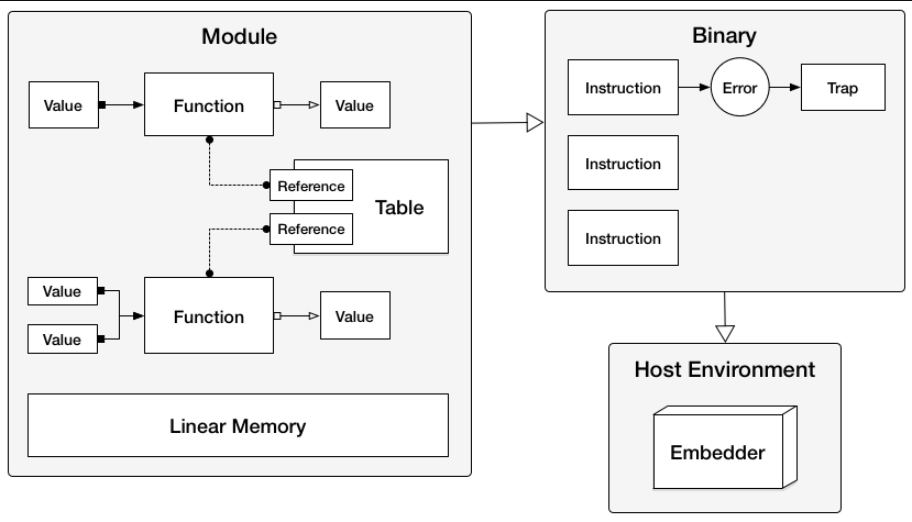
\includegraphics[width=0.9\columnwidth]{images/wasmArchitecture.png}
        \end{center}
        \caption{Architettura di WebAssembly}
        \label{fig:wasmArch}
\end{figure}

\newpage
\subsection{Le fasi semantiche}
Nella semantica di WebAssembly è possibile individuare tre fasi: decodifica, validazione ed esecuzione.
\subsubsection{Decodifica}
I moduli WebAssembly sono distribuiti in formato binario (.wasm) e per questo è necessario decodificarli in modo da ottenere una rappresentazione interna del modulo, con cui il web browser o il runtime environment potrà lavorare.
\subsubsection{Validazione}
Dopo aver decodificato i moduli binari, per poterli istanziare, è necessario verificare che questi siano validi.
La validità è appurata grazie ad un sistema di tipi basato sulla sintassi astratta di un modulo e sul suo contenuto. In particolare per ogni componente della sintassi è presente una regola che specifica le condizioni da rispettare perchè il modulo risulti valido.
!!!!Ad esempio viene controllato l'ordine delle istruzioni nel corpo di una funzione assicurandosi che lo stack sia utilizzato nel modo corretto.
Per esempio, dato un contesto \(C\) e un'istruzione del tipo \emph{t.binop} (che rappresenta un'operazione binaria tra tipi numerici, come ad esempio i32.add, f64.xor etc.) è valida con tipo \([t~t]{\rightarrow} [t]\), in notazione formale: 
\begin{equation*}
\frac{
}{
        C {\vdash} t\mathsf{.}{\mathit{binop}} : [t~t] {\rightarrow} [t]
}
\end{equation*}
Oppure con un'istruzione più complicata per l'aumento di memoria lineare \emph{memory.grow}:
\begin{itemize}
        \item La memoria \(C.{\mathit{mems}}[0]\) deve essere definita nel contesto.
        \item Allora l'istruzione risulta valida con tipo \([{\mathit{i32}}] {\rightarrow} [{\mathit{i32}}]\)
\end{itemize}
\begin{equation*}
        \frac{
        C.{\mathit{mems}}[0] = {\mathit{memtype}}
      }{
        C {\vdash} {\mathit{memory.grow}} : [{\mathit{i32}}] {\rightarrow} [{\mathit{i32}}]
      }        
\end{equation*}
\subsubsection{Esecuzione}
Terminata la validazione di ogni istruzione il modulo può finalmente essere istanziato.
L'istanza di un modulo ne è la rappresentazione dinamica. Esso comprende lo stack, sul quale operano le istruzioni WebAssembly e uno \emph{store} astratto, contenente lo stato globale (è la rappresentazione a runtime di tutte le istanze di funzioni, tabelle, memorie etc. che sono state allocate dall'istanziazione).
Terminata l'istanziazione, diventa effettivamente possibile l'esecuzione di istruzioni WebAssembly.
\\In particolare se nel modulo era stata definita una funzione \emph{\_start}, essa sarà eseguita subito dopo la creazione dell'istanza. D'ora in avanti diventerà anche possibile invocare funzioni esportate, chiamandole direttamente dall'istanza.
Per ogni istruzione , è presente una regola che specifica l'effetto della sua esecuzione sullo stato del programma. Rimanendo coerenti con gli esempi sulla validazione, segue il comportamento dell'istruzione \({\mathsf{t.binop}}\):
\begin{itemize}
        \item Grazie alla validazione assumiamo che due valori di tipo \(t\) siano in cima allo stack.
        \item Viene eseguita l'operazione di \textbf{pop} del valore \(t.const~c_1\) dallo stack
        \item Viene eseguita l'operazione di \textbf{pop} del valore \(t.const~c_2\) dallo stack
        \item Se \({\mathit{binop}}_t(c_1, c_2)\) è definita allora:
        \begin{itemize}
                \item Sia \(c\) il possibile risultato di \({\mathit{binop}}_t(c_1, c_2)\)
                \item Viene eseguita l'operazione di \textbf{push} del valore \(t.const~c\) nello stack
        \end{itemize}
        \item Altrimenti:
        \begin{itemize}
                \item Trap
        \end{itemize}
\end{itemize}
\begin{equation*}
        \begin{split}\begin{array}{lcl@{\qquad}l}
                (t\mathsf{.}{\mathsf{const}}~c_1)~(t\mathsf{.}{\mathsf{const}}~c_2)~t\mathsf{.}{\mathit{binop}} &{\hookrightarrow}& (t\mathsf{.}{\mathsf{const}}~c)
                  & (\mathrel{\mbox{if}} c \in {\mathit{binop}}_t(c_1,c_2)) \\
                (t\mathsf{.}{\mathsf{const}}~c_1)~(t\mathsf{.}{\mathsf{const}}~c_2)~t\mathsf{.}{\mathit{binop}} &{\hookrightarrow}& {\mathsf{trap}}
                  & (\mathrel{\mbox{if}} {\mathit{binop}}_{t}(c_1,c_2) = \{\})
                \end{array}\end{split}
\end{equation*}
Si noti che sia l'istanziazione, che l'invocazione di funzioni, sono operazioni che avvengono all'interno dell'ambiente di esecuzione dell'host.
\begin{figure}
        \begin{center}
                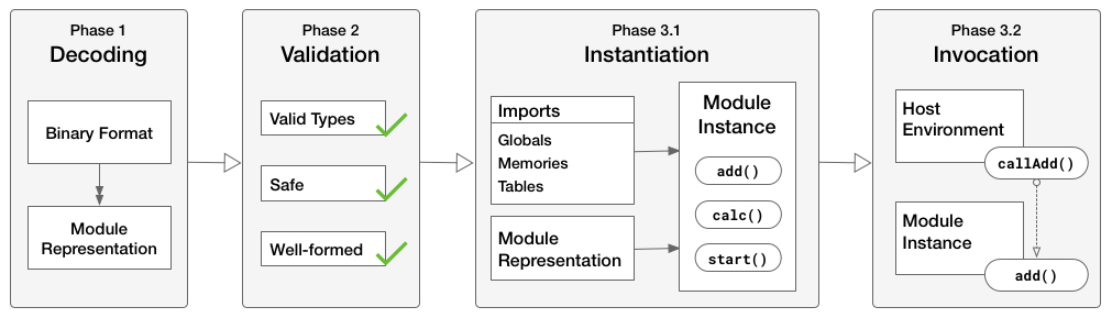
\includegraphics[width=0.97\columnwidth]{images/wasmSemanticPhases.png}
        \end{center}
        \caption{La semantica di WebAssembly}
        \label{fig:wasmPhases}
\end{figure}

\newpage
\subsection{Vantaggi di WebAssembly}
WebAssembly is being created as an open standard inside the W3C WebAssembly Community Group with the following goals:
Be fast, efficient, and portable — WebAssembly code can be executed at near-native speed across different platforms by taking advantage of common hardware capabilities.
Be readable and debuggable — WebAssembly is a low-level assembly language, but it does have a human-readable text format (the specification for which is still being finalized) that allows code to be written, viewed, and debugged by hand.
Keep secure — WebAssembly is specified to be run in a safe, sandboxed execution environment. Like other web code, it will enforce the browser's same-origin and permissions policies.
Don't break the web — WebAssembly is designed so that it plays nicely with other web technologies and maintains backwards compatibility.


\newpage
\section{WebAssembly System Interface}
\label{sec:WASI}
\subsection{Ruolo di WebAssembly System Interface}
\subsection{Rust e WASI}
\subsection{Struttura di WASI}
\subsection{Wasmtime}
\subsection{Applicazioni e Casistiche d'Uso di WASI}

\newpage
\section{Node.js}
\label{sec:Node}
\subsection{Panoramica di Node.js}
\subsection{Vantaggi di Node.js}
\subsection{Ecosistema di Node.js}

\newpage
\section{Confronto tra tecnologie}
\label{sec:Confronto}
\subsection{Prestazioni}
\subsection{Sicurezza}
\subsection{Facilità di Sviluppo}
\subsection{Scalabilità ed Espandibilità}

\newpage
\section{Conclusioni preliminari}
\label{sec:ConclusioniTecnologie}

\newpage
\lstinputlisting[label=lst:hello, firstline=2, lastline=4, caption={I directly included a portion of a file}]{code/hello.py}

\begin{lstlisting}[language=Java, label=lst:java, caption={Some code in another language than the default one}]
public void prepare(AClass foo) {
        AnotherClass bar = new AnotherClass(foo)
}
\end{lstlisting}
